\section{Scalability Bug Observations}

% example
To begin our work on combating scalability bugs, we start by conducting a study
to see their nature and how critical they are.
%
We perform a study of
\totAll scalability bugs reported from the deployments
of popular large-scale systems such as
Hadoop,
HBase,
HDFS,
Cassandra,
Couchbase,
Riak, and
Voldemort.
%
From the study, we observed many challenges in finding, reproducing, and
debugging scalability bugs. For example, let us consider a bug in Cassandra, a
highly-scalable peer-to-peer key-value store. If a user decommissions a single
node from a cluster of 50 nodes, the operation can be done smoothly. However, if
the user decommissions a node from a cluster of 200 nodes, the protocol that
re-calculate the key-range partitions (which nodes should own which key ranges)
becomes CPU intensive as the calculation has an $O(N^3)$ complexity where $N$ is
the number of nodes.  This combined with the gossiping and failure detection
logic leads to a scalability bug that makes the cluster unstable (many live
nodes are declared as dead, making some data not reachable by the users). We
give a full detail of the Cassandra bug in Section \ref{mot-bug}.

%
As in the example above, bug symptoms sometimes surface only in large deployment
scales (\eg, $N$$>$100 nodes), hence small/medium-scale testing is not enough.
Yet, not all developers have large test budgets, and even when they do,
debugging on hundreds of nodes is time consuming and difficult.
%
Furthermore, protocol algorithms can be scalable in the design sketches, but not
necessarily in the real deployments; there are specific implementation details
whose implications at scale are hard to predict. We discuss more about our
observations on scalability bugs in Section \ref{mot-observe}.

\subsection{A Sample Cassandra Bug}
\label{mot-bug}

\begin{figure}

\centerline{
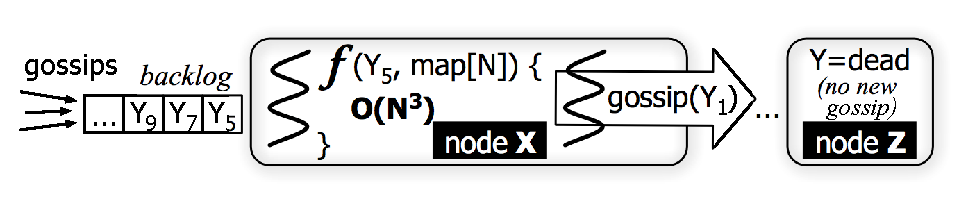
\includegraphics[height=0.8in]{F/cass1.eps}
%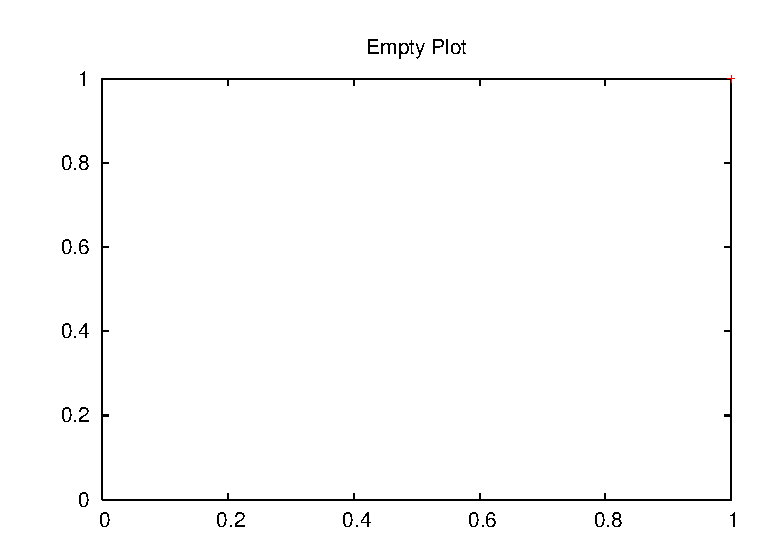
\includegraphics[height=0.6in]{F/empty.eps}
}
\vminfive
\mycaption{fig-cass1}{The problem of
gossip-based failure detection in Cassandra}{}
\vminfive
\end{figure}



We now describe in detail a scalability bug in Cassandra, which we use as a
sample bug.
%
Our journey in understanding scalability bugs began when we observed repeated
``flapping'' problems in large-scale Cassandra deployments (\ie, hundreds of
nodes).
%
Flapping is a cluster instability problem where node's up/down status
continuously flaps.  A ``flap'' is when a node X marks a peer node Y as down
(and soon marks Y as alive again).
%
We rigorously study a series of Cassandra bugs below that surfaced as the code
evolved.

%
%The bug surfaced on a cluster with hundreds of nodes and led to
%``\textit{\textbf{flapping}}'' nodes, a condition where node up/down status
%continuously changes;  tens of thousands of flaps\footnote{A ``\textbf{flap}''
%is when a node X marks a peer node Y as down.}  were observed.

To understand this bug, we need to understand the following protocols.

\begin{enumerate}

\item {\bf Bootstrap:} Each node first creates partition keys (\eg, 32 random
numbers) and gossips this information to peer nodes.
 
\item {\bf Gossip broadcast:} {\em Every second}, each node gossips to one
random node about a list of nodes and partitions it knows (including itself)
and their {\em version} numbers.  Each node also increments its version number
(``I'm still alive'') before gossiping.
 
\item {\bf Gossip processing:} The receiving node then finds any state
(metadata) differences between the two nodes to synchronize their views of the
ring.  Eventually, all nodes know about each other.
 
\item {\bf Failure detection:} {\em Every second}, a failure detection daemon
runs \cite{Lakshman+09-Cassandra}.  Put simply, if a node X has not received a
new gossip about Y {\em from anyone} (Y's version has not changed after some
period of time), X will declare Y dead (a flap).  When X receives a new gossip
about Y, it marks Y alive.

\end{enumerate}

% about the bug
There are two factors that induce the bug. The first is the {\em long latency
of scale-dependent state-update gossip processing during bootstrapping} (``f''
in Figure \ref{fig-cass1}).  While gossip processing is usually fast in a
stable cluster, it is expensive during bootstrapping as the gossips carry many
new state changes about the ring; the state-update processing time is
scale-dependent (\ie, greater than $O(N^3)$); the larger the cluster ($N$), the
larger the ring map, the longer the processing time is.
%
This long latency is caused by {\bf (1)} state-update checkpoint to on-disk
database and {\bf (2)} multi-map cloning and updates.
%
The first one is needed for fast fault tolerance; after a node crashes, it can
reboot fast as it knows the latest view of the ring.
%
The second one is preferred for simplicity; Cassandra clones its \ts{MultiMap}
ring table and applies changes one by one to alleviate long write locks.
%
% in order to prevent a long write lock on the ring table which can block other
% user-facing protocols.

% long
The second factor is the {\em single threaded} implementation of gossip
processing. As shown in Figure \ref{fig-cass1},  this inability to process
multiple gossips/state updates concurrently (for the sake of preventing
concurrency bugs) creates a {\em backlog} of new gossips.  For example, in {\em
every second}, Y tells someone it's alive with increasing version number (\eg,
Y$_7$), but the receiving nodes are still busy processing state changes and
only forward Y's old version number (\eg, Y$_1$).  As Y's new gossip is not
propagated on time,  other nodes (\eg, Z) will mark Y as dead.  This happens to
all nodes, not just Y.

% \ca{3831} -------------------------------------------------
The journey starts with Bug \#\ca{3831} \cite{CA-Two}, when a node D is
decommissioned from a cluster ring, D initiates a gossip telling that all other
nodes must rebalance the ring's key-ranges.  This scale-dependent ``pending
key-range calculation'' is CPU intensive with
%
% $O((n^2)log(n))$   % OLD
$O(MN^3log^3(N))$  % Tanakorn
%
complexity; $M$~is the list of key-range changes in the gossip message.  This
in turn leaves many gossips not propagated on time, creating flapping symptoms
that only appear at scale (at 200+ nodes; \sec\ref{sec-eval}). The developers
then optimized the code to
%
% $O(nlog(n))$  % OLD
$O(MN^2log^2(N))$ complexity.



% \ca{3881} -------------------------------------------------
Soon afterwards (Bug \#\ca{3881} \cite{CA-Tri}), Cassandra added the concept of
virtual partitions/nodes (\eg, $P$$=$$256$ per physical node).  As an
implication, the fix above did not scale as ``$N$'' becomes $N$$\times$$P$.
%
The bug was fixed with a complete redesign of the pending key-range
calculation, making it
% $O(log(N))$ OLD
$O(MNPlog^2(NP))$.

% \ca{5456} -------------------------------------------------
About a year later (\ca{5456} \cite{CA-Four}), Cassandra code employs
multi-threading between the pending key-range calculation and the gossip
processing with a coarse-grained lock to protect sharing of the ring
table.  Unbeknownst to the developers, at scale, the key-range calculation
can acquire the lock for a long time, causing flapping to reappear again.
The fix clones the ring table for the key-range calculation, to release the
lock early.



% \ca{6127} -------------------------------------------------
Later on (\ca{6127} \cite{CA-One}), a similar bug reappeared.  In the above
cases, the problems appeared when the cluster grows/shrinks gradually.
However, if user bootstrap a large cluster (\eg, 500+ nodes) from
scratch (\ie, all nodes do not know each other, with no established
key ranges),
%
the execution traverses a different code path that
performs a fresh ring-table/key-range construction with
$O(MN^2)$ % KORN
complexity.

% \tl{and there is no existing data stored in   the cluster}), 
% \tl{the offending function becomes the keyrange construction} 
%
% keyrange calculation which clones the ring table (a
% \ts{MultiMap}) becomes very expensive.  
%
% Including the cloning $O(N*P)$, we observed an 
% $O(N^3)$  $O(MN^2)$ % KORN complexity.

% ...............
The story continues on (\ca{6345}, \ca{6409}, \etc).  Fast forward today,
Cassandra developers recently started a new umbrella ticket for discussing
``Gossip 2.0,''  supposedly scalable to 1000+
nodes \cite{Gossip20, Gossip20Mail}.
% ---- 
Similar to Cassandra, other large-scale systems are prone to the same
problem.  So far, we have collected and analyzed \totCass Cassandra, \totCouch
Couchbase, \totHadoop Hadoop, \totHBase HBase, \totHDFS HDFS, \totRiak
Riak, and \totVold Voldemort scalability bugs, all caused user-visible
impacts.
%
This manual mining was arduous because there is no searchable jargon for
``scalability bugs''; we might have missed other bugs.
%

\section{Observations}
\label{mot-observe}

From the bug in previous section and all the bugs we studied, we make several
important observations.
%  regarding control-plane scalability bugs and distributed system designs.

\begin{itemize}
% only appear in large scale .. 
\item {\em Only appear at extreme scale:} \caone does not surface in 30-node
deployment.  In 128-node cluster, the symptom appears mildly (tens of
flaps).  From 200-500 nodes, flapping skyrockets from hundreds to 
thousands of flaps.  Testing in small/medium scales is not sufficient,
which is also true for other bugs we studied (\sec\ref{sec-eval}).





% theory is not enough
\item {\em Scalable in design, but not in practice.}  Related to \caone,
the accrual failure detector/gossiper
\cite{Hayashibara+04-PhiFailureDetector} was interestingly adopted by
Cassandra as it is scalable in design \cite{Lakshman+09-Cassandra}.
However, the design proof does not account gossip processing time during
bootstrap, which can be long.  To understand the bug, the developers tried
to ``do the [simple] math'' \cite{CA-One} but failed.  In practice, the
assumption that new gossips are propagated every second is not met (due to
the backlog).  The actual implementations overload gossips with many other
purposes (\eg, announcing boot/rebalance changes) beyond their original
design sketch.



% deep
\item {\em Implementation specific and hard to predict.}  The
backlog-induced flapping in \caone was caused specifically by Cassandra's
implementation choice: metadata checkpoint, multi-map cloning, and its
single-threaded implementation.  State-update processing time is hard to
predict (ranges from 0.001 to 4 seconds) as it depends on a 2-dimensional
input: the receiving node's ring table size and the number of new
state changes (\sec\ref{sec-eval}).

% a two-dimensional input; more in \sec\ref{sec-eval}).  

% not independent
\item {\em Cascading impacts of ``not-so-independent'' nodes.}  In 
cluster-wide control protocols, distributed nodes are  not
necessarily independent; nodes must communicate with each other
to synchronize their views of cluster metadata.  As the cluster grows, the
cluster metadata size increases.  Thus, unpredictable processing time in
individual nodes can create cascading impacts to the whole cluster.


% 
\item {\em Long and difficult large-scale debugging:} 
%
The bug report of \caone generated over 40 back-and-forth discussion
comments and took 2 months to fix.  It is apparent \cite{CA-One} that
there were many hurdles of deploying and debugging the buggy protocol at
real scale.  Important to note is that debugging is {\em not} a single
iteration; developers must {\em repeatedly} instrument the system (add
more logs) and re-run the system at scale to find and fix the bug, which
is not trivial.  The scalability bugs we studied took 6 to 157 days to
fix (27 on average).


\item {\em Not all developers have large test budgets:}
%
Another factor of delayed fixes is the lack of budget for large
test clusters.  Such luxury tends to be accessible to developers 
in large companies, but not to 
open-source developers.  When
\caone was submitted by a customer who had hundreds of nodes, the
Cassandra developers did not have an instant access to a test cluster of
the same scale.



% repeated 
\item {\em Quick fixes and repeated bugs:} Bugs are often fixed with quick
patches (development pressures), but the new fix might not eradicate the
problem completely \cite{Yin+11-FixesBecomeBugs}.
%
For example, for \caone, the patch simply disables failure detection during
bootstrap.  As the protocol was not redesigned, the bug still appeared in
another workload (\eg, scaling out from 128 to 256 nodes).
%
In the latest Cassandra, the simple fix has been removed and the gossip
protocol has been redesigned.
%
We also found that old fixes can become obsolete in 
protocol re-designs, which then can give birth to new scalability bugs. 
%
For example, the fix for \ca{3831} became obsolete as ``vnodes'' was
introduced, which then gave rise to a new 
vnode-related scalability bug
(\ca{3881}).
%
A scale-check could have ensured that new fixes remove old scalability bugs
entirely and similar bugs do not re-surface in new designs.
\end{itemize}


\if 0
Our observations above accentuate the need for scale-checking distributed
system {\em implementations} at {\em real scale}, not via simulation nor
extrapolation.  In this context, we now discuss the state of the art.
\fi

